% Options for packages loaded elsewhere
\PassOptionsToPackage{unicode}{hyperref}
\PassOptionsToPackage{hyphens}{url}
\PassOptionsToPackage{dvipsnames,svgnames,x11names}{xcolor}
%
\documentclass[
  letterpaper,
  DIV=11,
  numbers=noendperiod]{scrartcl}

\usepackage{amsmath,amssymb}
\usepackage{lmodern}
\usepackage{iftex}
\ifPDFTeX
  \usepackage[T1]{fontenc}
  \usepackage[utf8]{inputenc}
  \usepackage{textcomp} % provide euro and other symbols
\else % if luatex or xetex
  \usepackage{unicode-math}
  \defaultfontfeatures{Scale=MatchLowercase}
  \defaultfontfeatures[\rmfamily]{Ligatures=TeX,Scale=1}
\fi
% Use upquote if available, for straight quotes in verbatim environments
\IfFileExists{upquote.sty}{\usepackage{upquote}}{}
\IfFileExists{microtype.sty}{% use microtype if available
  \usepackage[]{microtype}
  \UseMicrotypeSet[protrusion]{basicmath} % disable protrusion for tt fonts
}{}
\makeatletter
\@ifundefined{KOMAClassName}{% if non-KOMA class
  \IfFileExists{parskip.sty}{%
    \usepackage{parskip}
  }{% else
    \setlength{\parindent}{0pt}
    \setlength{\parskip}{6pt plus 2pt minus 1pt}}
}{% if KOMA class
  \KOMAoptions{parskip=half}}
\makeatother
\usepackage{xcolor}
\usepackage[normalem]{ulem}
\setlength{\emergencystretch}{3em} % prevent overfull lines
\setcounter{secnumdepth}{-\maxdimen} % remove section numbering
% Make \paragraph and \subparagraph free-standing
\ifx\paragraph\undefined\else
  \let\oldparagraph\paragraph
  \renewcommand{\paragraph}[1]{\oldparagraph{#1}\mbox{}}
\fi
\ifx\subparagraph\undefined\else
  \let\oldsubparagraph\subparagraph
  \renewcommand{\subparagraph}[1]{\oldsubparagraph{#1}\mbox{}}
\fi

\usepackage{color}
\usepackage{fancyvrb}
\newcommand{\VerbBar}{|}
\newcommand{\VERB}{\Verb[commandchars=\\\{\}]}
\DefineVerbatimEnvironment{Highlighting}{Verbatim}{commandchars=\\\{\}}
% Add ',fontsize=\small' for more characters per line
\usepackage{framed}
\definecolor{shadecolor}{RGB}{241,243,245}
\newenvironment{Shaded}{\begin{snugshade}}{\end{snugshade}}
\newcommand{\AlertTok}[1]{\textcolor[rgb]{0.68,0.00,0.00}{#1}}
\newcommand{\AnnotationTok}[1]{\textcolor[rgb]{0.37,0.37,0.37}{#1}}
\newcommand{\AttributeTok}[1]{\textcolor[rgb]{0.40,0.45,0.13}{#1}}
\newcommand{\BaseNTok}[1]{\textcolor[rgb]{0.68,0.00,0.00}{#1}}
\newcommand{\BuiltInTok}[1]{\textcolor[rgb]{0.00,0.23,0.31}{#1}}
\newcommand{\CharTok}[1]{\textcolor[rgb]{0.13,0.47,0.30}{#1}}
\newcommand{\CommentTok}[1]{\textcolor[rgb]{0.37,0.37,0.37}{#1}}
\newcommand{\CommentVarTok}[1]{\textcolor[rgb]{0.37,0.37,0.37}{\textit{#1}}}
\newcommand{\ConstantTok}[1]{\textcolor[rgb]{0.56,0.35,0.01}{#1}}
\newcommand{\ControlFlowTok}[1]{\textcolor[rgb]{0.00,0.23,0.31}{#1}}
\newcommand{\DataTypeTok}[1]{\textcolor[rgb]{0.68,0.00,0.00}{#1}}
\newcommand{\DecValTok}[1]{\textcolor[rgb]{0.68,0.00,0.00}{#1}}
\newcommand{\DocumentationTok}[1]{\textcolor[rgb]{0.37,0.37,0.37}{\textit{#1}}}
\newcommand{\ErrorTok}[1]{\textcolor[rgb]{0.68,0.00,0.00}{#1}}
\newcommand{\ExtensionTok}[1]{\textcolor[rgb]{0.00,0.23,0.31}{#1}}
\newcommand{\FloatTok}[1]{\textcolor[rgb]{0.68,0.00,0.00}{#1}}
\newcommand{\FunctionTok}[1]{\textcolor[rgb]{0.28,0.35,0.67}{#1}}
\newcommand{\ImportTok}[1]{\textcolor[rgb]{0.00,0.46,0.62}{#1}}
\newcommand{\InformationTok}[1]{\textcolor[rgb]{0.37,0.37,0.37}{#1}}
\newcommand{\KeywordTok}[1]{\textcolor[rgb]{0.00,0.23,0.31}{#1}}
\newcommand{\NormalTok}[1]{\textcolor[rgb]{0.00,0.23,0.31}{#1}}
\newcommand{\OperatorTok}[1]{\textcolor[rgb]{0.37,0.37,0.37}{#1}}
\newcommand{\OtherTok}[1]{\textcolor[rgb]{0.00,0.23,0.31}{#1}}
\newcommand{\PreprocessorTok}[1]{\textcolor[rgb]{0.68,0.00,0.00}{#1}}
\newcommand{\RegionMarkerTok}[1]{\textcolor[rgb]{0.00,0.23,0.31}{#1}}
\newcommand{\SpecialCharTok}[1]{\textcolor[rgb]{0.37,0.37,0.37}{#1}}
\newcommand{\SpecialStringTok}[1]{\textcolor[rgb]{0.13,0.47,0.30}{#1}}
\newcommand{\StringTok}[1]{\textcolor[rgb]{0.13,0.47,0.30}{#1}}
\newcommand{\VariableTok}[1]{\textcolor[rgb]{0.07,0.07,0.07}{#1}}
\newcommand{\VerbatimStringTok}[1]{\textcolor[rgb]{0.13,0.47,0.30}{#1}}
\newcommand{\WarningTok}[1]{\textcolor[rgb]{0.37,0.37,0.37}{\textit{#1}}}

\providecommand{\tightlist}{%
  \setlength{\itemsep}{0pt}\setlength{\parskip}{0pt}}\usepackage{longtable,booktabs,array}
\usepackage{calc} % for calculating minipage widths
% Correct order of tables after \paragraph or \subparagraph
\usepackage{etoolbox}
\makeatletter
\patchcmd\longtable{\par}{\if@noskipsec\mbox{}\fi\par}{}{}
\makeatother
% Allow footnotes in longtable head/foot
\IfFileExists{footnotehyper.sty}{\usepackage{footnotehyper}}{\usepackage{footnote}}
\makesavenoteenv{longtable}
\usepackage{graphicx}
\makeatletter
\def\maxwidth{\ifdim\Gin@nat@width>\linewidth\linewidth\else\Gin@nat@width\fi}
\def\maxheight{\ifdim\Gin@nat@height>\textheight\textheight\else\Gin@nat@height\fi}
\makeatother
% Scale images if necessary, so that they will not overflow the page
% margins by default, and it is still possible to overwrite the defaults
% using explicit options in \includegraphics[width, height, ...]{}
\setkeys{Gin}{width=\maxwidth,height=\maxheight,keepaspectratio}
% Set default figure placement to htbp
\makeatletter
\def\fps@figure{htbp}
\makeatother

\KOMAoption{captions}{tableheading}
\makeatletter
\makeatother
\makeatletter
\makeatother
\makeatletter
\@ifpackageloaded{caption}{}{\usepackage{caption}}
\AtBeginDocument{%
\ifdefined\contentsname
  \renewcommand*\contentsname{Table of contents}
\else
  \newcommand\contentsname{Table of contents}
\fi
\ifdefined\listfigurename
  \renewcommand*\listfigurename{List of Figures}
\else
  \newcommand\listfigurename{List of Figures}
\fi
\ifdefined\listtablename
  \renewcommand*\listtablename{List of Tables}
\else
  \newcommand\listtablename{List of Tables}
\fi
\ifdefined\figurename
  \renewcommand*\figurename{Figure}
\else
  \newcommand\figurename{Figure}
\fi
\ifdefined\tablename
  \renewcommand*\tablename{Table}
\else
  \newcommand\tablename{Table}
\fi
}
\@ifpackageloaded{float}{}{\usepackage{float}}
\floatstyle{ruled}
\@ifundefined{c@chapter}{\newfloat{codelisting}{h}{lop}}{\newfloat{codelisting}{h}{lop}[chapter]}
\floatname{codelisting}{Listing}
\newcommand*\listoflistings{\listof{codelisting}{List of Listings}}
\makeatother
\makeatletter
\@ifpackageloaded{caption}{}{\usepackage{caption}}
\@ifpackageloaded{subcaption}{}{\usepackage{subcaption}}
\makeatother
\makeatletter
\@ifpackageloaded{tcolorbox}{}{\usepackage[many]{tcolorbox}}
\makeatother
\makeatletter
\@ifundefined{shadecolor}{\definecolor{shadecolor}{rgb}{.97, .97, .97}}
\makeatother
\makeatletter
\makeatother
\ifLuaTeX
  \usepackage{selnolig}  % disable illegal ligatures
\fi
\IfFileExists{bookmark.sty}{\usepackage{bookmark}}{\usepackage{hyperref}}
\IfFileExists{xurl.sty}{\usepackage{xurl}}{} % add URL line breaks if available
\urlstyle{same} % disable monospaced font for URLs
\hypersetup{
  pdftitle={Práctica 1. Introducción a R y RStudio},
  pdfauthor={Jesús Martín Fernández},
  colorlinks=true,
  linkcolor={blue},
  filecolor={Maroon},
  citecolor={Blue},
  urlcolor={Blue},
  pdfcreator={LaTeX via pandoc}}

\title{{Práctica 1. Introducción a R y RStudio}}
\author{Jesús Martín Fernández}
\date{}

\begin{document}
\maketitle
\ifdefined\Shaded\renewenvironment{Shaded}{\begin{tcolorbox}[frame hidden, interior hidden, boxrule=0pt, borderline west={3pt}{0pt}{shadecolor}, sharp corners, breakable, enhanced]}{\end{tcolorbox}}\fi

\renewcommand*\contentsname{Contenidos}
{
\hypersetup{linkcolor=}
\setcounter{tocdepth}{3}
\tableofcontents
}
\hypertarget{section}{%
\subsection{}\label{section}}

\hypertarget{quuxe9-es-r-y-cuxf3mo-funciona-r}{%
\subsection{1. ¿Qué es R y cómo funciona
R?}\label{quuxe9-es-r-y-cuxf3mo-funciona-r}}

R es un lenguaje de programación y un entorno de software creado con el
propósito de facilitar el análisis estadístico, la visualización de
datos y la manipulación de información en distintos formatos. Desde su
origen, se ha consolidado como una de las herramientas más utilizadas en
disciplinas como la estadística, la ciencia de datos, las ciencias de la
salud, la economía y muchas otras áreas que requieren un manejo
intensivo de datos.

A diferencia de otros lenguajes de programación que necesitan compilar
el código en un archivo ejecutable antes de poder utilizarlo, R es un
lenguaje interpretado. Esto significa que el usuario puede escribir y
ejecutar instrucciones de manera interactiva, observando los resultados
de forma inmediata sin pasar por un proceso de compilación previo. Esta
característica favorece la experimentación, ya que permite probar
diferentes enfoques, realizar ajustes rápidos y explorar conjuntos de
datos con mayor agilidad.

Además, R cuenta con una amplia comunidad que ha desarrollado miles de
paquetes adicionales, lo que amplía enormemente sus capacidades. Estos
paquetes permiten realizar desde análisis estadísticos avanzados hasta
la creación de gráficos altamente personalizados, integrando incluso
técnicas modernas de aprendizaje automático y minería de datos.

Gracias a esta combinación de flexibilidad, interactividad y ecosistema
colaborativo, R se ha convertido en una herramienta indispensable tanto
para quienes se inician en el análisis de datos, como es nuestro caso,
como para profesionales que trabajan en proyectos de investigación o en
aplicaciones prácticas de gran escala.

\hypertarget{un-poco-de-historia}{%
\subsubsection{1.1 Un poco de historia}\label{un-poco-de-historia}}

La historia de \textbf{R} comienza en 1992, cuando Robert Gentleman y
Ross Ihaka, del Departamento de Estadística de la Universidad de
Auckland (Nueva Zelanda), iniciaron el desarrollo de un nuevo lenguaje
de programación orientado al análisis estadístico. Sin embargo, sus
orígenes se remontan más atrás, ya que R tiene sus raíces en el
\textbf{lenguaje S}, creado a finales de los años setenta por John
Chambers y su equipo en los Laboratorios Bell (hoy Alcatel-Lucent) en
Nueva Jersey. El nombre ``S'', abreviatura de statistics, hacía alusión
al célebre lenguaje C ---también desarrollado en Bell Labs--- y fue
diseñado para facilitar el análisis de datos, sentando las bases de
muchas de las herramientas estadísticas modernas.

Con el paso del tiempo, S fue evolucionando y eventualmente se
comercializó bajo el nombre \textbf{S-Plus}, al añadírsele una interfaz
gráfica de usuario (GUI). No obstante, la aparición de R marcaría un
punto de inflexión: no solo retomaba las fortalezas de S, sino que
incorporaba elementos del lenguaje \textbf{Scheme}, lo que le otorgaba
mayor flexibilidad en la gestión de objetos y estructuras. Según sus
creadores, ``el lenguaje resultante es muy similar en apariencia a S,
pero en su semántica de fondo deriva de Scheme''. El nombre \textbf{R}
fue elegido en parte como homenaje a S, y en parte por la inicial de los
nombres de sus desarrolladores.

En sus primeras etapas, R se distribuía como software experimental. La
versión 0.16, una versión alfa, ya incluía varias de las funcionalidades
descritas en el llamado White Book de S. En 1997, apareció la versión
0.49, la más antigua cuyo código aún se conserva y que podía compilarse
en sistemas UNIX. Ese mismo año se fundó el \textbf{CRAN (Comprehensive
R Archive Network)} con tres servidores espejo y apenas doce paquetes.
También en 1997, R fue adoptado como parte del \textbf{Proyecto GNU},
consolidando su condición de software libre y comenzando a gestionarse
con el sistema CVS, lo que permitió un desarrollo más colaborativo y
organizado.

El avance de R fue constante. En el año 2000 se lanzó la versión 1.0.0,
considerada la primera estable para su uso en producción. Luego se
añadieron innovaciones importantes: los métodos S4 en la versión 1.4.0,
el soporte para UTF-8 en la versión 2.1.0 y el sistema de lazy loading
en la 2.0.0, que mejoró la eficiencia en la carga de datos. Con la
llegada de la versión 2.11.0, R amplió su soporte a Windows de 64 bits,
y en versiones posteriores se optimizó la internacionalización y la
velocidad de serialización. La versión 3.0.0, publicada en abril de
2013, introdujo mejoras en la interfaz gráfica, en la gestión de memoria
y en el rendimiento general. Posteriormente, la versión \textbf{3.4.0}
(2017) habilitó por defecto el compilador \textbf{JIT (Just-In-Time)} en
nivel 3, lo que supuso un salto notable en velocidad de ejecución.

En paralelo, mientras S y S-Plus quedaban relegados, R fue ganando
terreno por dos razones fundamentales: era gratuito y contaba con una
comunidad cada vez más amplia que contribuía activamente a su expansión.
Por este motivo, en ocasiones se le ha denominado GNU S, en
reconocimiento a su naturaleza de software libre y a su vínculo con el
Proyecto GNU.

Hoy en día, R sigue siendo mantenido por el \textbf{R Development Core
Team} y se ha consolidado como una de las herramientas más influyentes
en la estadística, la ciencia de datos y la investigación aplicada. Sin
embargo, su éxito no se debe únicamente a sus características técnicas,
sino también a la comunidad global de usuarios y desarrolladores que lo
rodea. Esta red ha impulsado la creación de miles de paquetes, guías,
foros y proyectos colaborativos que enriquecen continuamente el
ecosistema de R, asegurando que siga siendo una plataforma viva,
innovadora y en constante evolución.

\uline{La Comunidad R}

La comunidad global de R no solo está formada por usuarios, sino también
por contribuyentes que desarrollan paquetes para la biblioteca CRAN y
brindan apoyo en foros y plataformas. Es conocida por su dinamismo y
compromiso, donde sus miembros gestionan foros, escriben blogs
especializados y responden preguntas en Stack Overflow, creando una
sólida red de soporte.

Además, la comunidad organiza conferencias sobre R en todo el mundo,
ofreciendo oportunidades para aprender, compartir conocimientos y
conectar con otros profesionales y entusiastas.

Si estás comenzando con R, seguramente encontrarás un paquete que se
ajuste a tus necesidades. La comunidad ha desarrollado miles de
herramientas que amplían las capacidades de R, con CRAN albergando casi
20.000 paquetes.

\hypertarget{cuxf3mo-funciona-r}{%
\subsubsection{1.2 Cómo funciona R}\label{cuxf3mo-funciona-r}}

R trabaja con objetos (variables, datos, funciones, resultados) que se
almacenan en la memoria activa y se manipulan mediante operadores y
funciones. Los resultados también son objetos que pueden analizarse. Los
archivos solo se usan para entrada y salida de datos, mientras que las
funciones se organizan en paquetes, con el paquete base como núcleo para
tareas clave de manipulación de datos y análisis estadístico. Los
operadores en R son intuitivos, y las funciones, que también son
objetos, permiten realizar análisis complejos. La sintaxis accesible y
su estructura orientada a objetos hacen de R una herramienta eficaz para
el análisis de datos.

A diferencia de los programas tradicionales que muestran inmediatamente
los resultados, R almacena los resultados como objetos, lo que permite
al usuario trabajar con ellos más tarde. Por ejemplo, si se está
analizando una gran base de datos y se construyen una decena de modelos
explicativos de los cuáles solo se quiere elegir uno, R guarda el objeto
que contiene toda la información de cada modelo. En lugar de mostrar
todos los detalles de cada uno de ellos inmediatamente, se puede extraer
solo la bondad de ajuste o los coeficientes de cada modelo, sin tener
que lidiar con una salida masiva de información. Esto hace que R sea más
flexible y eficiente en el manejo de datos complejos.

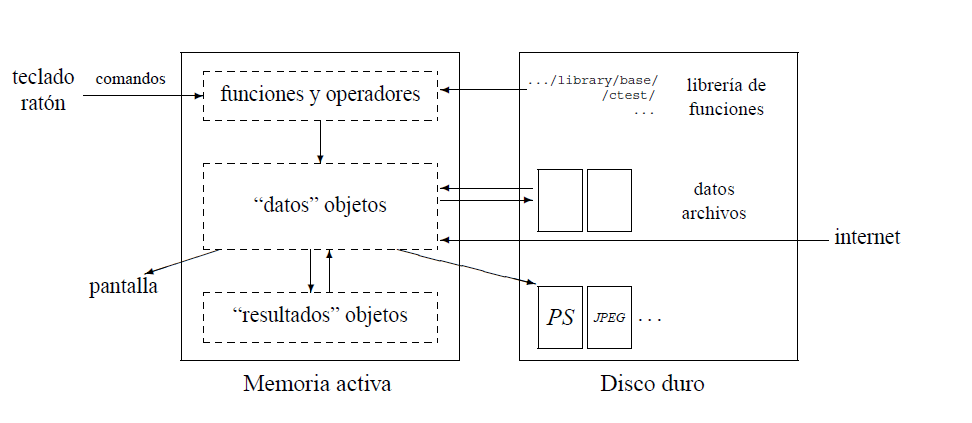
\includegraphics{images/clipboard-988688670.png}

Esquema del funcionamiento de R (tomado de Paradis, E. (2005).~ \emph{R
for Beginners}. Institut des Sciences de l'Evolution. Université
Montpellier II.)

Otra de las ventajas de R es su sintaxis sencilla, que permite a los
usuarios realizar operaciones y análisis complejos de manera intuitiva.
A diferencia de otros lenguajes de programación que requieren
estructuras más elaboradas, R utiliza comandos directos que facilitan el
trabajo desde el principio, lo que permite a los usuarios centrarse en
el análisis sin preocuparse demasiado por la complejidad técnica.

Además, R es consistente en el uso de las funciones, todas las funciones
en R deben incluir paréntesis, lo que crea una estructura clara y
predecible. Esta característica asegura que los usuarios sepan
exactamente cómo interactuar con cada función, independientemente de si
reciben o no argumentos. Si se omiten los paréntesis, en lugar de
ejecutar la función, R muestra su definición interna, lo que permite a
los usuarios ver y entender cómo está diseñada.

Este enfoque estructurado y accesible de R fomenta tanto el aprendizaje
rápido como la exploración más profunda del código. Los usuarios pueden
comenzar realizando operaciones básicas, pero también tienen la libertad
de explorar cómo se construyen las funciones y modificarlas si es
necesario, lo que convierte a R en una herramienta altamente flexible
para el análisis de datos.

\hypertarget{comenzando-a-trabajar-con-r}{%
\subsection{2. Comenzando a trabajar con
R}\label{comenzando-a-trabajar-con-r}}

\hypertarget{instalaciuxf3n-de-r}{%
\subsubsection{2.1 Instalación de R}\label{instalaciuxf3n-de-r}}

Para instalar R vamos a la página web de~R project:
\href{http://www.r-project.org/}{\textbf{http://www.r-project.org}}\textbf{.}


\includegraphics{Imagenes/CRAN_2.jpeg}

Después seleccionamos el ``espejo'' más conveniente, en nuestro país una
opción adecuada está en la Red Iris The Comprehensive R Archive Network
(rediris.es) \url{https://cran.rediris.es/}. Allí nos descargaremos el
formato conveniente en función del sistema operativo.

En el entorno de la URJC lo tenemos operativo en MyApps
\url{https://myapps.urjc.es/myapps/Apps}

Al instalar R, el \textbf{paquete base} se incluye automáticamente. Este
paquete proporciona herramientas esenciales para manipular datos,
realizar cálculos estadísticos y crear gráficos. No es necesario
instalarlo por separado, ya que está disponible desde el inicio para que
puedas empezar a trabajar con R de inmediato.

\hypertarget{rstudio-una-interfaz-para-usar-r}{%
\subsubsection{2.2 RStudio: una interfaz para usar
R}\label{rstudio-una-interfaz-para-usar-r}}

Aunque puedes ejecutar R directamente desde la línea de comandos,
\textbf{RStudio} es una interfaz gráfica que facilita el uso de R,
especialmente para principiantes.

RStudio se descarga desde su página oficial
\url{https://www.rstudio.com/}

Pero también puedes encontrarla en MyApps

Esta es la apariencia de RStudio

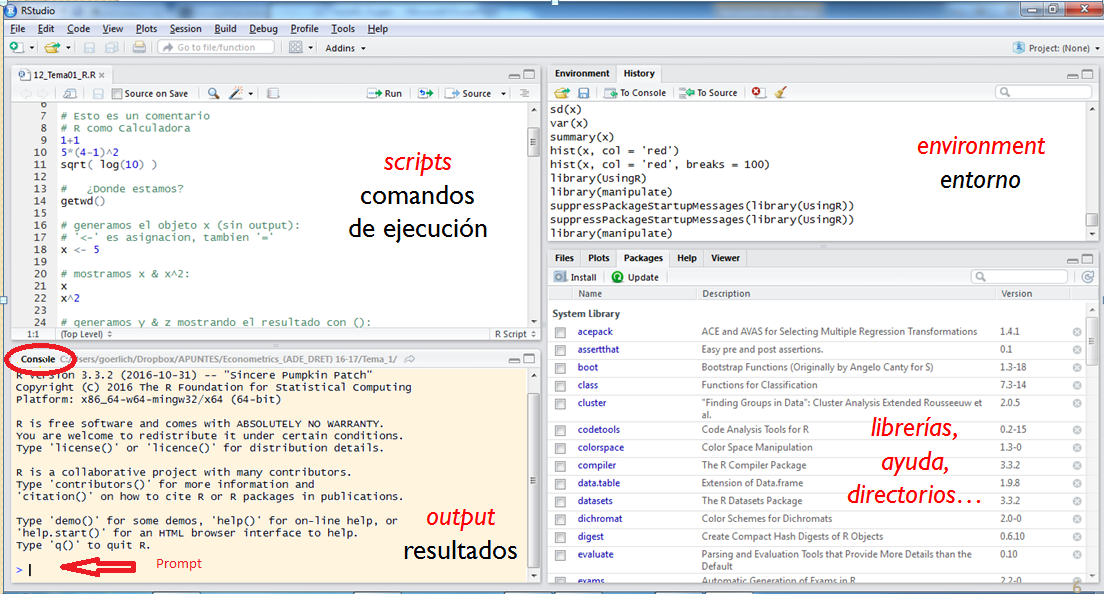
\includegraphics{Imagenes/Rstudio_consola.png}

En RStudio, la \textbf{consola} se encuentra por defecto en el panel
inferior izquierdo, en la pestaña etiquetada como Console. Aquí es donde
interactuamos directamente con R. Debajo de esta pestaña, verás un texto
introductorio seguido del símbolo ``\textgreater{}'', que indica que R
está listo para recibir instrucciones. En esta consola puedes escribir
comandos o código, y al pulsar Enter, R ejecutará el comando y mostrará
el resultado inmediatamente en la misma consola. Es el lugar principal
para ejecutar scripts de manera interactiva y ver resultados en tiempo
real.

Escribe esta operación en la consola y mira el resultado

\begin{Shaded}
\begin{Highlighting}[]
\DecValTok{3}\SpecialCharTok{+}\DecValTok{2}
\end{Highlighting}
\end{Shaded}

\begin{verbatim}
[1] 5
\end{verbatim}

También pueden introducirse órdenes diversas en la consola en líneas
sucesivas o separadas por el símbolo \texttt{;}

\begin{Shaded}
\begin{Highlighting}[]
\DecValTok{3}\SpecialCharTok{+}\DecValTok{2} 
\end{Highlighting}
\end{Shaded}

\begin{verbatim}
[1] 5
\end{verbatim}

\begin{Shaded}
\begin{Highlighting}[]
\DecValTok{2}\SpecialCharTok{*}\NormalTok{(}\DecValTok{4{-}1}\NormalTok{)}\SpecialCharTok{\^{}}\DecValTok{2} 
\end{Highlighting}
\end{Shaded}

\begin{verbatim}
[1] 18
\end{verbatim}

\begin{Shaded}
\begin{Highlighting}[]
\FunctionTok{log10}\NormalTok{ (}\DecValTok{100}\NormalTok{) }
\end{Highlighting}
\end{Shaded}

\begin{verbatim}
[1] 2
\end{verbatim}

\begin{Shaded}
\begin{Highlighting}[]
\FunctionTok{sqrt}\NormalTok{(}\DecValTok{36}\NormalTok{)}
\end{Highlighting}
\end{Shaded}

\begin{verbatim}
[1] 6
\end{verbatim}

\begin{Shaded}
\begin{Highlighting}[]
\DecValTok{3}\SpecialCharTok{+}\DecValTok{2}\NormalTok{ ; }\DecValTok{2}\SpecialCharTok{*}\NormalTok{(}\DecValTok{4{-}1}\NormalTok{)}\SpecialCharTok{\^{}}\DecValTok{2}\NormalTok{ ; }\FunctionTok{log10}\NormalTok{ (}\DecValTok{100}\NormalTok{) ;}\FunctionTok{sqrt}\NormalTok{(}\DecValTok{36}\NormalTok{)}
\end{Highlighting}
\end{Shaded}

\begin{verbatim}
[1] 5
\end{verbatim}

\begin{verbatim}
[1] 18
\end{verbatim}

\begin{verbatim}
[1] 2
\end{verbatim}

\begin{verbatim}
[1] 6
\end{verbatim}

En RStudio, el panel de \textbf{script} se encuentra en la parte
superior izquierda, permitiendo escribir y ejecutar instrucciones línea
por línea o en bloque, igual que en la Consola. Para ejecutar el código,
puedes optar por varias alternativas: hacer clic en el botón
\textbf{Run} en la parte derecha del panel de script, o puedes usar el
atajo \textbf{Ctrl+Enter.}

Los contenidos del panel script pueden guardarse usando \textbf{File
\textgreater{} Save as..} y seleccionar la ruta deseada, o haciendo clic
en el botón \textbf{Guardar} en la cinta de opciones del script.

El panel de \textbf{Entorno} en RStudio está dividido en dos pestañas
principales: \textbf{Environment} y \textbf{History} (otra denominada
Connection no la explicaremos de momento)

En la pestaña \textbf{Environment}, se muestran todos los objetos (como
variables, data frames, y otros elementos) que has creado durante tu
sesión de trabajo. Aquí también puedes gestionar tu sesión de trabajo
mediante opciones como cargar y guardar el estado actual, importar datos
y limpiar los objetos de la sesión. Estas funciones son accesibles a
través de la cinta de opciones situada en esta pestaña, facilitando la
administración de tus datos y objetos.

La pestaña \textbf{History} registra todas las instrucciones que has
ejecutado. Además de mostrar un historial completo de los comandos
utilizados, te permite gestionar este historial de manera eficiente.
Puedes cargar y guardar el historial de comandos, seleccionar uno o
varios comandos y enviarlos a la consola o al script para su
re-ejecución. También puedes limpiar el historial cuando ya no lo
necesites. Esta pestaña es útil para revisar y reutilizar comandos
anteriores, lo que facilita el trabajo continuo y la replicación de
análisis.

El panel habitualmente situado en el cuadrante inferior derecho
contiene, a su vez, varias pestañas.

Entre las pestañas destacadas se encuentran:

\begin{itemize}
\item
  \textbf{Files}: Actúa como un explorador de archivos, permitiendo la
  navegación y gestión de los archivos en el sistema.
\item
  \textbf{Plots}: Muestra los gráficos generados durante la sesión. En
  esta pestaña, se pueden utilizar opciones como \textbf{Zoom} para
  ampliar los gráficos en una ventana separada, y \textbf{Export} para
  guardar los gráficos en formatos de imagen, PDF, o copiarlos al
  portapapeles.
\item
  \textbf{Packages}: Ofrece un listado de los paquetes instalados en R y
  aquellos que están cargados en la sesión actual. Desde esta pestaña,
  se pueden instalar nuevos paquetes, así como actualizar los ya
  existentes.
\item
  \textbf{Help}: Proporciona asistencia sobre funciones específicas,
  facilitando la consulta de documentación y ayuda relacionada con el
  uso de diversas funciones en R.
\end{itemize}

\hypertarget{establecer-el-directorio-de-trabajo}{%
\subsubsection{2.3 Establecer el directorio de
trabajo}\label{establecer-el-directorio-de-trabajo}}

Antes de empezar a trabajar en R, debes fijar el directorio donde se
guardarán tus archivos. Hay dos maneras de hacerlo:

\begin{enumerate}
\def\labelenumi{\arabic{enumi}.}
\item
  \textbf{Fijar el directorio manualmente}: Usa la función
  \texttt{setwd("C:/ruta\ del\ directorio\ de\ trabajo")} para
  establecer la ruta de trabajo. Para verificar la ruta actual, usa
  \texttt{getwd()}, y para listar los archivos en el directorio, utiliza
  \texttt{dir()}.
\item
  \textbf{Crear un proyecto de R}: Selecciona \textbf{File
  \textgreater{} New Project\ldots{}} para vincular todos los archivos
  al proyecto. Puedes crear un nuevo directorio con un proyecto vacío o
  elegir una carpeta existente. Al crear el proyecto, se genera un
  archivo \texttt{.Rproj}, y todos los archivos asociados se guardarán
  en la carpeta del proyecto. Para abrir un proyecto, haz doble clic en
  el archivo \texttt{.Rproj} o selecciona \textbf{File \textgreater{}
  Open Project\ldots{}} en RStudio.
\end{enumerate}

Los proyectos facilitan la organización, ya que todos los archivos
creados se guardan automáticamente en la carpeta del proyecto.

Es importante como se debe indicar la ruta de cualquier archivo en R. En
la navegación de archivos y rutas en sistemas operativos, el uso de
barras invertidas (\texttt{\textbackslash{}}) y barras normales
(\texttt{/}) tiene diferentes significados según el entorno.

Cuando se trabaja en \textbf{R} y \textbf{RStudio}, se debe tener en
cuenta que \textbf{R} utiliza barras normales (\texttt{/}) en las rutas
de archivos . Sin embargo, si estás escribiendo rutas en
\textbf{Windows} y usas barras invertidas (\texttt{\textbackslash{}}),
(como hace Windows habitualmente) recuerda que en \textbf{R} se debe
duplicar cada barra invertida para que se interprete correctamente, es
decir, podras escibir

\texttt{C:/Users/Usuario/Documents/Archivo.txt}. o

\texttt{C:\textbackslash{}\textbackslash{}Users\textbackslash{}\textbackslash{}Usuario\textbackslash{}\textbackslash{}Documents\textbackslash{}\textbackslash{}Archivo.txt}.

\hypertarget{instalaciuxf3n-y-uso-de-paquetes}{%
\subsubsection{2.4 Instalación y uso de
paquetes}\label{instalaciuxf3n-y-uso-de-paquetes}}

Un paquete es un conjunto de funciones, datos y documentación que están
organizados para realizar tareas específicas. \textbf{R} viene con
algunos paquetes preinstalados, pero puedes descargar e instalar muchos
más desde repositorios en línea o desde archivos locales en tu
computadora. Para la instalación desde repositorios necesitarás una
conexión a Internet, pero puedes hacerlo desde directorios locales si ya
tienes el archivo del paquete en tu computadora.

\uline{Paquetes base}

Los paquetes ``base'' ya vienen preinstalados con \textbf{R} y se pueden
cargar directamente usando la función \texttt{library()}. Por ejemplo:

\begin{Shaded}
\begin{Highlighting}[]
\FunctionTok{library}\NormalTok{(}\StringTok{"stats"}\NormalTok{)}
\end{Highlighting}
\end{Shaded}

Este comando carga el paquete \texttt{stats}, el cual es parte de la
instalación base y proporciona funciones estadísticas comunes.

\uline{Otros paquetes}

Para utilizar paquetes adicionales disponibles en \textbf{CRAN}, deben
realizarse dos pasos: la instalación y la carga.

La instalación se realiza mediante la función
\texttt{install.packages()}, y la carga posterior se realiza con
\texttt{library()}. Por ejemplo, para instalar y cargar el paquete
\texttt{ggplot2}, se haría lo siguiente:

\begin{Shaded}
\begin{Highlighting}[]
\FunctionTok{install.packages}\NormalTok{ (}\StringTok{"ggplot2"}\NormalTok{)   }
\FunctionTok{library}\NormalTok{(}\StringTok{"ggplot2"}\NormalTok{)           }
\end{Highlighting}
\end{Shaded}

Es importante entender que las funciones de un paquete no están
disponibles hasta que el paquete ha sido cargado explícitamente con
\texttt{library()}. Esto es para mejorar la eficiencia del sistema y
evitar conflictos de espacio de nombres, es decir, evitar que dos
funciones con el mismo nombre de diferentes paquetes interfieran entre
sí. Si alguna vez una función no se ejecuta, y funcionó en el pasado, es
recomendable verificar si el paquete correspondiente ha sido cargado.

Para saber que un paquete está instalado se puede usar la función
\texttt{find()}

\begin{Shaded}
\begin{Highlighting}[]
\FunctionTok{find.package}\NormalTok{(}\StringTok{"ggplot2"}\NormalTok{)}
\end{Highlighting}
\end{Shaded}

\begin{verbatim}
[1] "C:/Users/Usuario/Documents/GitHub/med_pr2025_book/renv/library/windows/R-4.4/x86_64-w64-mingw32/ggplot2"
\end{verbatim}

Finalmente, si un paquete ya no es necesario, puede ser removido con
\texttt{remove.packages()}, liberando espacio y manteniendo el entorno
de trabajo más organizado.

\begin{Shaded}
\begin{Highlighting}[]
\FunctionTok{remove.packages}\NormalTok{(}\StringTok{"ggplot2"}\NormalTok{)}
\end{Highlighting}
\end{Shaded}

\uline{Estructura de los paquetes en R}

Una vez instalado, un paquete se guarda en una carpeta específica dentro
del directorio R HOME/library, que es el directorio donde R está
instalado. Cada paquete contiene sus funciones organizadas en
subdirectorios. Por ejemplo, el paquete base (parte del núcleo de R)
está ubicado en \texttt{R\ HOME/library/base/R/base}, y contiene un
archivo en formato ASCII que incluye todas las funciones del paquete.

\hypertarget{la-ayuda-en-r}{%
\subsubsection{2.5 La ayuda en R}\label{la-ayuda-en-r}}

Existen diversas formas de buscar ayuda en R

\begin{itemize}
\tightlist
\item
  \texttt{help(función)} o \texttt{?función}: Ayuda para una función.
\end{itemize}

\begin{Shaded}
\begin{Highlighting}[]
\FunctionTok{help}\NormalTok{(mean)}
\NormalTok{?mean}
\end{Highlighting}
\end{Shaded}

\begin{itemize}
\tightlist
\item
  \texttt{args(función)}: Argumentos de una función.
\end{itemize}

\begin{Shaded}
\begin{Highlighting}[]
\FunctionTok{args}\NormalTok{(mean)}
\end{Highlighting}
\end{Shaded}

\begin{verbatim}
function (x, ...) 
NULL
\end{verbatim}

\begin{itemize}
\tightlist
\item
  \texttt{help(package\ =\ "paquete")}: Documentación del paquete.
\end{itemize}

\begin{Shaded}
\begin{Highlighting}[]
\FunctionTok{help}\NormalTok{(}\AttributeTok{package =} \StringTok{"ggplot2"}\NormalTok{)}
\end{Highlighting}
\end{Shaded}

Muestra la documentación del paquete ggplot2.

\begin{itemize}
\tightlist
\item
  \texttt{vignette(package=)}:
\end{itemize}

\begin{Shaded}
\begin{Highlighting}[]
\FunctionTok{vignette}\NormalTok{(}\AttributeTok{package =} \StringTok{"ggplot2"}\NormalTok{)}
\end{Highlighting}
\end{Shaded}

Muestra vignettes de \texttt{ggplot2}

Las vignettes en R son documentos extensos que proporcionan una visión
detallada y práctica sobre cómo usar un paquete, sus funciones y sus
características. A menudo incluyen ejemplos, tutoriales, y descripciones
de cómo aplicar el paquete para resolver problemas específicos. Las
vignettes son una forma útil de aprender sobre un paquete y cómo
aprovecharlo al máximo.

\begin{itemize}
\tightlist
\item
  \texttt{help.search("término")} o \texttt{??"término"}:
\end{itemize}

\begin{Shaded}
\begin{Highlighting}[]
\FunctionTok{help.search}\NormalTok{(}\StringTok{"plot"}\NormalTok{) }
\NormalTok{??plot}
\end{Highlighting}
\end{Shaded}

Busca en la ayuda de R.

Existen otras funciones de ayuda en R

\begin{itemize}
\item
  \texttt{search()}: Muestra los objetos y paquetes actualmente cargados
  en la sesión de R.
\item
  \texttt{data()}: Lista los conjuntos de datos disponibles en los
  paquetes cargados.
\item
  \texttt{available.packages()}: Muestra todos los paquetes disponibles
  en el repositorio CRAN o el repositorio establecido con
  \texttt{setRepositories()}.
\item
  \texttt{installed.packages()}: Lista los paquetes instalados en todas
  las bibliotecas especificadas en \texttt{.libPaths()}, proporcionando
  más detalles que \texttt{library()}.
\item
  \texttt{help(package="ggplot2")}: Proporciona ayuda sobre el paquete
  \texttt{ggplot2}, mostrando la documentación general del paquete.
\item
  \texttt{help(ggplot,\ package="ggplot2")}: Ofrece ayuda sobre la
  función \texttt{ggplot} dentro del paquete \texttt{ggplot2}, útil
  cuando varias funciones tienen el mismo nombre en diferentes paquetes.
\item
  \texttt{library(help="dplyr")}: Muestra la documentación del paquete
  \texttt{dplyr} en un formato diferente.
\item
  \texttt{package?dplyr}: Muestra una descripción del paquete
  \texttt{dplyr}, aunque no todos los paquetes tienen documentación
  accesible de esta manera.
\item
  \texttt{ls("package:tidyr")}: Lista las funciones y objetos
  disponibles en el paquete \texttt{tidyr}, que debe estar cargado en la
  sesión.
\end{itemize}

Recuerda que en RStudio en el panel de la parte inferior derecha hay
también una pestaña de ayuda con un buscador de términos

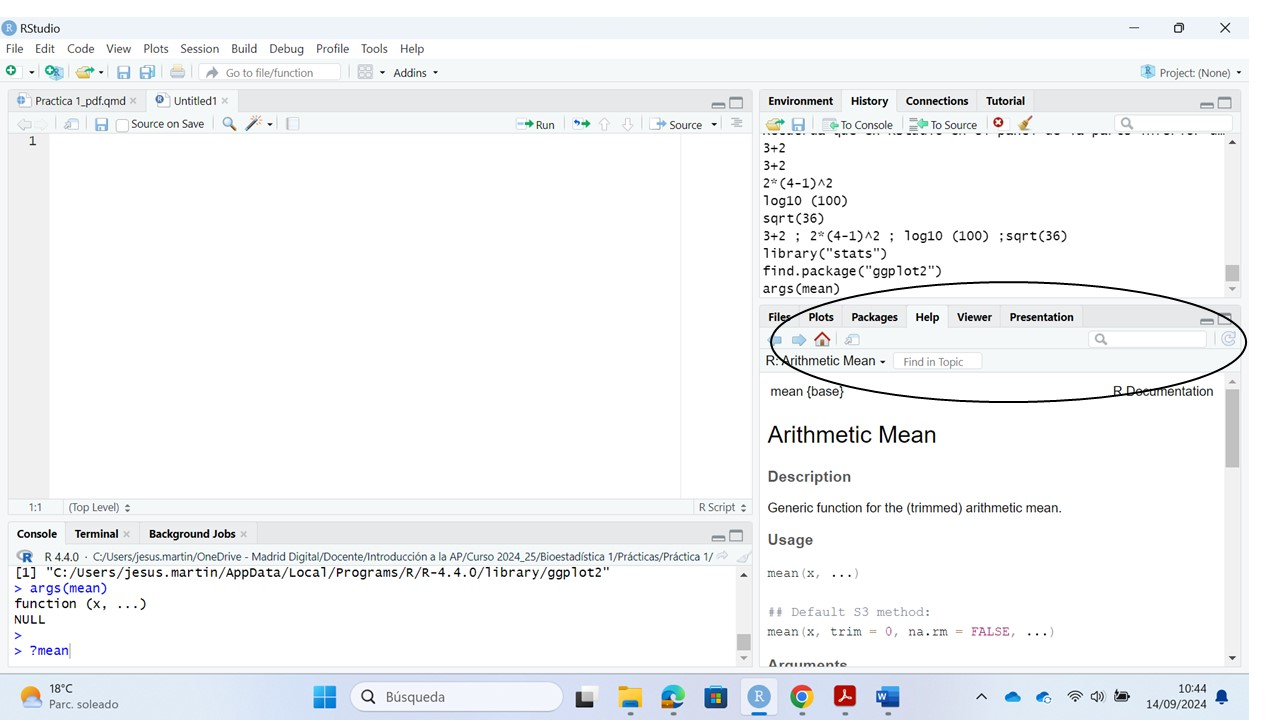
\includegraphics{Imagenes/Ayuda RStudio.jpg}

\hypertarget{operando-con-r.}{%
\subsection{3. Operando con R.}\label{operando-con-r.}}

En \textbf{R}, el lenguaje es \textbf{case-sensitive}, lo que significa
que distingue entre mayúsculas y minúsculas, haciendo que
\texttt{Variable}, \texttt{variable}, y \texttt{VARIABLE} se consideren
nombres distintos. Los nombres de objetos no pueden contener espacios;
en su lugar, se deben usar guiones bajos (\texttt{\_}) o la notación de
camello (\texttt{camelCase}) para separar palabras (esto último lo
usamos menos). Además, los nombres deben comenzar con una letra o un
punto seguido de una letra, y pueden incluir letras, números, y puntos o
guiones bajos después del primer carácter. Nombres que comienzan con
números o que contienen espacios o caracteres especiales generarán
errores.

Los caracteres reservados como \texttt{=}, \texttt{\$}, \texttt{\&}, y
\texttt{*}, así como caracteres especiales como \texttt{ä}, \texttt{ü},
\texttt{í}, no están permitidos en los nombres de objetos, ya que pueden
causar errores o comportamientos inesperados.

\hypertarget{las-luxedneas-de-cuxf3digo-en-r}{%
\subsubsection{3.1 Las líneas de código en
R}\label{las-luxedneas-de-cuxf3digo-en-r}}

En R, como ya señalamos, los comandos se pueden separar por punto y coma
(\texttt{;}) o por saltos de línea. Esto permite flexibilidad en cómo se
estructuran y escriben los comandos en el código. Por ejemplo:

\begin{Shaded}
\begin{Highlighting}[]
\NormalTok{x }\OtherTok{\textless{}{-}} \DecValTok{10}\NormalTok{; y }\OtherTok{\textless{}{-}} \DecValTok{20}\NormalTok{; z }\OtherTok{\textless{}{-}}\NormalTok{ x }\SpecialCharTok{+}\NormalTok{ y}
\end{Highlighting}
\end{Shaded}

Crea los mismos objetos que

\begin{Shaded}
\begin{Highlighting}[]
\NormalTok{x }\OtherTok{\textless{}{-}} \DecValTok{10}
\NormalTok{y }\OtherTok{\textless{}{-}} \DecValTok{20}
\NormalTok{z }\OtherTok{\textless{}{-}}\NormalTok{ x }\SpecialCharTok{+}\NormalTok{ y}
\end{Highlighting}
\end{Shaded}

Además, R permite que el código se escriba en varias líneas y se agrupen
bloques de código usando llaves (\texttt{\{\}}). Esto es especialmente
útil para definir funciones, estructuras de control , o simplemente para
organizar el código en secciones claras. Por ejemplo:

\begin{Shaded}
\begin{Highlighting}[]
\NormalTok{\{}
\NormalTok{  x }\OtherTok{\textless{}{-}} \DecValTok{5}
\NormalTok{  y }\OtherTok{\textless{}{-}}\NormalTok{ x }\SpecialCharTok{*} \DecValTok{2}
  \FunctionTok{print}\NormalTok{(y)}
\NormalTok{\}}
\end{Highlighting}
\end{Shaded}

\begin{verbatim}
[1] 10
\end{verbatim}

Los comentarios en R se introducen con el símbolo \texttt{\#}. Todo lo
que sigue a este símbolo en una línea se considera un comentario y no se
ejecuta. Los comentarios no afectan la ejecución del código, pero hacen
que sea más fácil entender y mantener el código en el futuro. Por
ejemplo:

\begin{Shaded}
\begin{Highlighting}[]
\CommentTok{\# Este es un comentario}
\NormalTok{x }\OtherTok{\textless{}{-}} \DecValTok{10}  \CommentTok{\# Asignamos 10 a x}
\NormalTok{y }\OtherTok{\textless{}{-}} \DecValTok{20}  \CommentTok{\# Asignamos 20 a y}

\CommentTok{\# Calculamos la suma}
\NormalTok{z }\OtherTok{\textless{}{-}}\NormalTok{ x }\SpecialCharTok{+}\NormalTok{ y}
\NormalTok{z}
\end{Highlighting}
\end{Shaded}

\begin{verbatim}
[1] 30
\end{verbatim}

\hypertarget{creaciuxf3n-de-objetos-con-r}{%
\subsubsection{3.2 Creación de objetos con
R}\label{creaciuxf3n-de-objetos-con-r}}

En \textbf{R}, los objetos se crean y asignan utilizando el operador
\texttt{\textless{}-}, que es la forma más común de asignar valores a
variables. Los objetos pueden tener diferentes tipos de datos, como
numérico, carácter, lógico o complejo, y cada uno tiene atributos que
definen su naturaleza y tamaño. Por ejemplo, puedes crear un objeto
numérico asignando un valor entero o decimal a una variable, como
\texttt{x\ \textless{}-\ 1} o \texttt{y\ \textless{}-\ 3.14}.

\begin{Shaded}
\begin{Highlighting}[]
\NormalTok{x}\OtherTok{\textless{}{-}}\DecValTok{1} 
\NormalTok{x }
\end{Highlighting}
\end{Shaded}

\begin{verbatim}
[1] 1
\end{verbatim}

\begin{Shaded}
\begin{Highlighting}[]
\NormalTok{y}\OtherTok{\textless{}{-}}\FloatTok{3.14}
\NormalTok{y}
\end{Highlighting}
\end{Shaded}

\begin{verbatim}
[1] 3.14
\end{verbatim}

Del mismo modo, puedes crear un objeto carácter asignando una cadena de
texto, como \texttt{nombre\ \textless{}-\ "Juan"}.

\begin{Shaded}
\begin{Highlighting}[]
\NormalTok{nombre }\OtherTok{\textless{}{-}} \StringTok{"Juan"} 
\NormalTok{nombre}
\end{Highlighting}
\end{Shaded}

\begin{verbatim}
[1] "Juan"
\end{verbatim}

También existen objetos con valores lógicos . En \textbf{R}, un objeto
lógico es una variable que puede tener uno de dos valores posibles:
\texttt{TRUE} (verdadero) o \texttt{FALSE} (falso). Los valores lógicos
se utilizan para realizar operaciones de comparación, control de flujo
en el código, y para representar estados binarios o condiciones en tus
análisis.

\begin{Shaded}
\begin{Highlighting}[]
\NormalTok{numeros }\OtherTok{\textless{}{-}} \DecValTok{1}\SpecialCharTok{:}\DecValTok{5}  
\CommentTok{\# Crear un vector lógico que indica si los números son mayores que 3 }
\NormalTok{mayor\_que\_tres }\OtherTok{\textless{}{-}}\NormalTok{ numeros }\SpecialCharTok{\textgreater{}} \DecValTok{3}  
\CommentTok{\# Mostrar el vector lógico }
\FunctionTok{print}\NormalTok{(mayor\_que\_tres)}
\end{Highlighting}
\end{Shaded}

\begin{verbatim}
[1] FALSE FALSE FALSE  TRUE  TRUE
\end{verbatim}

Cada objeto tiene dos atributos principales: \textbf{tipo de dato} y
\textbf{longitud}. El tipo de dato indica la clase básica del objeto,
mientras que la longitud se refiere al número de elementos que contiene.

\begin{Shaded}
\begin{Highlighting}[]
\NormalTok{x }\OtherTok{\textless{}{-}}\NormalTok{ (}\DecValTok{1}\SpecialCharTok{:}\DecValTok{5}\NormalTok{) }
\NormalTok{A }\OtherTok{\textless{}{-}} \StringTok{"Australopitecus"}  
\CommentTok{\# Ver el tipo y longitud de los objetos }
\FunctionTok{mode}\NormalTok{(x)       }
\end{Highlighting}
\end{Shaded}

\begin{verbatim}
[1] "numeric"
\end{verbatim}

\begin{Shaded}
\begin{Highlighting}[]
\FunctionTok{length}\NormalTok{(x) }
\end{Highlighting}
\end{Shaded}

\begin{verbatim}
[1] 5
\end{verbatim}

\begin{Shaded}
\begin{Highlighting}[]
\FunctionTok{mode}\NormalTok{(A)       }
\end{Highlighting}
\end{Shaded}

\begin{verbatim}
[1] "character"
\end{verbatim}

\begin{Shaded}
\begin{Highlighting}[]
\FunctionTok{length}\NormalTok{(A)}
\end{Highlighting}
\end{Shaded}

\begin{verbatim}
[1] 1
\end{verbatim}

\textbf{R} también maneja valores especiales como \texttt{NA} (not
Available) para datos faltantes, \texttt{Inf} y \texttt{-Inf} para
infinito positivo y negativo, y \texttt{NaN\ (not\ a\ number)} para
resultados no válidos.

\begin{Shaded}
\begin{Highlighting}[]
\NormalTok{c}\OtherTok{\textless{}{-}}\FunctionTok{c}\NormalTok{(}\DecValTok{1}\NormalTok{,}\DecValTok{2}\NormalTok{,}\ConstantTok{NA}\NormalTok{,}\DecValTok{4}\NormalTok{,}\DecValTok{5}\NormalTok{) }
\NormalTok{c }
\end{Highlighting}
\end{Shaded}

\begin{verbatim}
[1]  1  2 NA  4  5
\end{verbatim}

\begin{Shaded}
\begin{Highlighting}[]
\DecValTok{1}\SpecialCharTok{/}\DecValTok{0} 
\end{Highlighting}
\end{Shaded}

\begin{verbatim}
[1] Inf
\end{verbatim}

\begin{Shaded}
\begin{Highlighting}[]
\SpecialCharTok{{-}}\DecValTok{1}\SpecialCharTok{/}\DecValTok{0}
\end{Highlighting}
\end{Shaded}

\begin{verbatim}
[1] -Inf
\end{verbatim}

\begin{Shaded}
\begin{Highlighting}[]
\DecValTok{0}\SpecialCharTok{/}\DecValTok{0}
\end{Highlighting}
\end{Shaded}

\begin{verbatim}
[1] NaN
\end{verbatim}

En la próxima práctica se explicarán con más detalle los tipos de
objetos en \textbf{R}.

Para listar los objetos en el entorno de trabajo en R, puedes utilizar
la función \texttt{ls()}, que proporciona una lista de todos los objetos
actualmente disponibles. También puedes usar \texttt{objects()}, que es
funcionalmente equivalente a \texttt{ls()}, o \texttt{ls.str()}, que
ofrece una vista más detallada de los objetos junto con información
sobre sus estructuras.

\begin{Shaded}
\begin{Highlighting}[]
\FunctionTok{ls}\NormalTok{()}
\end{Highlighting}
\end{Shaded}

\begin{verbatim}
[1] "A"              "c"              "mayor_que_tres" "nombre"        
[5] "numeros"        "x"              "y"              "z"             
\end{verbatim}

\begin{Shaded}
\begin{Highlighting}[]
\FunctionTok{objects}\NormalTok{ ()}
\end{Highlighting}
\end{Shaded}

\begin{verbatim}
[1] "A"              "c"              "mayor_que_tres" "nombre"        
[5] "numeros"        "x"              "y"              "z"             
\end{verbatim}

\begin{Shaded}
\begin{Highlighting}[]
\FunctionTok{ls.str}\NormalTok{()}
\end{Highlighting}
\end{Shaded}

\begin{verbatim}
A :  chr "Australopitecus"
c :  num [1:5] 1 2 NA 4 5
mayor_que_tres :  logi [1:5] FALSE FALSE FALSE TRUE TRUE
nombre :  chr "Juan"
numeros :  int [1:5] 1 2 3 4 5
x :  int [1:5] 1 2 3 4 5
y :  num 3.14
z :  num 30
\end{verbatim}

Finalmente los objetos se pueden borrar con las funciones \texttt{rm()},
que permite eliminar uno o varios objetos del entorno de trabajo. Si
deseas limpiar el entorno completamente, puedes usar
\texttt{rm(list\ =\ ls())} para borrar todos los objetos a la vez

\begin{Shaded}
\begin{Highlighting}[]
\FunctionTok{rm}\NormalTok{ (x)}
\FunctionTok{rm}\NormalTok{ (y,A)}
\FunctionTok{rm}\NormalTok{ (}\AttributeTok{list=} \FunctionTok{ls}\NormalTok{())}
\end{Highlighting}
\end{Shaded}

\hypertarget{las-funciones-en-r}{%
\subsubsection{3.3 Las funciones en R}\label{las-funciones-en-r}}

En \textbf{R}, las funciones son bloques de código reutilizables
diseñados para realizar tareas específicas y pueden ser una herramienta
poderosa en el análisis de datos. Cada función en \textbf{R} tiene una
estructura compuesta por tres partes principales: el nombre de la
función, los argumentos y las opciones.

El nombre de la función es el identificador que se utiliza para llamar a
la función, y debe ser único y descriptivo para facilitar su comprensión
y uso.

Los argumentos son los valores que se pasan a la función para que
realice su tarea, y pueden ser obligatorios o opcionales dependiendo de
cómo esté diseñada la función.

Las opciones son parámetros adicionales que permiten ajustar el
comportamiento de la función, ofreciendo flexibilidad para personalizar
su funcionamiento.

Por ejemplo, en la función \texttt{sum()}, que se utiliza para calcular
la suma de valores, el nombre de la función es \texttt{sum}, el
argumento principal es \texttt{...}, que representa los números a sumar,
y la opción \texttt{na.rm} permite decidir si se deben ignorar los
valores faltantes (\texttt{NA}).

\begin{Shaded}
\begin{Highlighting}[]
\NormalTok{x1 }\OtherTok{\textless{}{-}} \FunctionTok{c}\NormalTok{(}\DecValTok{1}\SpecialCharTok{:}\DecValTok{10}\NormalTok{, }\ConstantTok{NA}\NormalTok{, }\DecValTok{12}\SpecialCharTok{:}\DecValTok{20}\NormalTok{)}
\NormalTok{result1 }\OtherTok{\textless{}{-}} \FunctionTok{sum}\NormalTok{(x1, }\AttributeTok{na.rm =} \ConstantTok{TRUE}\NormalTok{)}
\NormalTok{result1}
\end{Highlighting}
\end{Shaded}

\begin{verbatim}
[1] 199
\end{verbatim}

\begin{Shaded}
\begin{Highlighting}[]
\NormalTok{x2 }\OtherTok{\textless{}{-}} \FunctionTok{c}\NormalTok{(}\DecValTok{1}\SpecialCharTok{:}\DecValTok{20}\NormalTok{)}
\NormalTok{result2 }\OtherTok{\textless{}{-}} \FunctionTok{sum}\NormalTok{(x2, }\AttributeTok{na.rm =} \ConstantTok{TRUE}\NormalTok{)}
\NormalTok{result2}
\end{Highlighting}
\end{Shaded}

\begin{verbatim}
[1] 210
\end{verbatim}

En \textbf{R}, las funciones son una herramienta fundamental para
estructurar el código de manera clara y eficiente. Al permitir que las
tareas complejas se dividan en bloques más manejables, las funciones
fomentan la modularidad, lo que facilita la reutilización del código y
reduce la duplicación. Esto no solo mejora la legibilidad y el
mantenimiento del código, sino que también optimiza el uso de recursos
tanto del programador como del sistema. Además, el uso de argumentos y
opciones dentro de las funciones brinda flexibilidad, permitiendo
personalizar su comportamiento según las necesidades del análisis, lo
que las convierte en un componente clave para escribir código adaptable
y robusto.

\hypertarget{guardando-el-trabajo-realizado}{%
\subsection{4. Guardando el trabajo
realizado}\label{guardando-el-trabajo-realizado}}

En RStudio, existen varias formas de \textbf{guardar tu trabajo}
dependiendo de lo que deseas conservar (scripts, resultados, gráficos,
etc.). Aquí se explican las principales opciones:

\uline{1. Guardar scripts o archivos de código R}

El código que escribes en el editor de scripts de RStudio (los archivos
con extensión \texttt{.R}) se puede guardar fácilmente como un archivo
de texto. Basta con ir al menú File \textgreater{} Save o usar el atajo
de teclado Ctrl + S (Windows)

\uline{2. \textbf{Guardar el entorno de trabajo (Workspace)}}

El entorno de trabajo incluye todos los objetos (variables, funciones,
data frames, etc.) que has creado durante una sesión de R. Para guardar
el entorno de trabajo ve a Session \textgreater{} Save Workspace
As\ldots{} y guarda el archivo con la extensión \texttt{.RData}. Esto
permitirá que, al abrir el archivo más tarde, recuperes todos los
objetos y variables tal como estaban al guardarlo. También puedes
guardar manualmente usando el comando \texttt{save.image()}, que guarda
el entorno actual en un archivo \texttt{.RData}:

\begin{Shaded}
\begin{Highlighting}[]
\FunctionTok{save.image}\NormalTok{(}\AttributeTok{file =} \StringTok{"mi\_trabajo.RData"}\NormalTok{) }
\end{Highlighting}
\end{Shaded}

Más tarde puede recuperarse mediante el uso de la función
\texttt{load()}

\begin{Shaded}
\begin{Highlighting}[]
\FunctionTok{load}\NormalTok{(}\StringTok{"mi\_trabajo.RData"}\NormalTok{) }
\end{Highlighting}
\end{Shaded}

\uline{3. Guardar un proyecto de RStudio}

Los proyectos en RStudio ayudan a organizar mejor el trabajo, creando un
entorno aislado con sus propios scripts, datos, y configuraciones. Se
pueden guardar en la pestaña Save Project As\ldots{} y guarda el
proyecto con la extensión \texttt{.Rproj}. Esto permite cargar todo el
entorno de trabajo, configuración, y scripts asociados con el proyecto
en el futuro.

\uline{4. Guardar gráficos}

Si has generado gráficos y deseas guardarlos, puedes hacerlo en varios
formatos como PNG, PDF, JPEG, etc. Para guardar un gráfico desde la
interfaz gráfica ve a la ventana de gráficos, haz clic en Export y
selecciona Save as Image o Save as PDF. Puedes elegir el formato y la
resolución. También puedes guardar un gráfico desde el código,
utilizando funciones como \texttt{png()}, \texttt{pdf()}, o
\texttt{jpeg()} antes de generar el gráfico.

\begin{Shaded}
\begin{Highlighting}[]
\FunctionTok{png}\NormalTok{(}\StringTok{"mi\_grafico.png"}\NormalTok{)}
\FunctionTok{plot}\NormalTok{(x, y)  }\CommentTok{\# Generar gráfico suponiendo que tenemos vectores x e y}
\FunctionTok{dev.off}\NormalTok{()  }\CommentTok{\# Cerrar el dispositivo gráfico}
\end{Highlighting}
\end{Shaded}

\uline{5. Guardar datos}

Si has trabajado con datos (por ejemplo un dataframe, ya veremos más
adelante) y deseas guardarlos en archivos externos (como CSV, Excel,
etc.), puedes hacerlo utilizando funciones específicas para escribir
archivos. En algunos casos hay que cargar previamente alguna librería,
por ejemplo para guardar un excel

\begin{Shaded}
\begin{Highlighting}[]
\FunctionTok{write.csv}\NormalTok{(mis\_datos, }\StringTok{"mis\_datos.csv"}\NormalTok{) }

\CommentTok{\#Para un formato excel}
\FunctionTok{library}\NormalTok{(writexl) }
\FunctionTok{write\_xlsx}\NormalTok{(mis\_datos, }\StringTok{"mis\_datos.xlsx"}\NormalTok{)}
\end{Highlighting}
\end{Shaded}

\hypertarget{recuperando-archivos}{%
\subsection{5. Recuperando archivos}\label{recuperando-archivos}}

A veces necesitamos volver a abrir un archivo o recuperar la ruta donde
guardamos nuestro trabajo en R. Para hacerlo de manera rápida, podemos
aprovechar el portapapeles de Windows y algunas funciones de R.

\textbf{Usando el portapapeles}

En Windows, la función \texttt{readClipboard()} permite leer
directamente lo que tenemos copiado en el portapapeles. Esto resulta
útil cuando copiamos la ruta de un archivo desde el explorador de
Windows y queremos usarla en R.

Por ejemplo, si copiamos la ruta de un archivo como:

\begin{Shaded}
\begin{Highlighting}[]
\CommentTok{\# Recuperar código desde el portapapeles}
\FunctionTok{readClipboard}\NormalTok{()}

\CommentTok{\#readClipboard() hace legible la ruta Windows en R (añade doble barra)}
\end{Highlighting}
\end{Shaded}

\textbf{Nota importante}:\\

Recordamos que Windows usa la barra invertida \texttt{\textbackslash{}}
en sus rutas, pero R requiere doble barra
\texttt{\textbackslash{}\textbackslash{}} o una barra normal \texttt{/}.
La función \texttt{readClipboard()} hace automáticamente la conversión,
lo cual facilita mucho el trabajo.

\textbf{Iniciando una sesión limpia y cargando el archivo}

Supongamos que previamente hemos trabajado en un script o sesión de R y
queremos recuperar nuestro trabajo rápidamente. Una forma de hacerlo es
copiando el código desde un archivo o desde el portapapeles y luego
ejecutarlo en R. Para esto, R ofrece la función
\texttt{readClipboard()}, que permite leer directamente lo que tenemos
copiado en el portapapeles.

Por ejemplo, imaginemos que copiamos nuestro código desde un archivo
llamado
\texttt{"C:\textbackslash{}\textbackslash{}\textasciitilde{}mi\_trabajo.RData"}
en Windows y queremos recuperarlo en R:

\begin{Shaded}
\begin{Highlighting}[]
\CommentTok{\# Recuperar código desde el portapapeles}
\FunctionTok{readClipboard}\NormalTok{()}

\CommentTok{\#readClipboard() hace legible la ruta Windows en R (añade doble barra)}

\CommentTok{\# Limpiar el entorno para empezar desde cero}
\FunctionTok{rm}\NormalTok{(}\AttributeTok{list =} \FunctionTok{ls}\NormalTok{())}

\CommentTok{\# Definir el directorio de trabajo}
\FunctionTok{setwd}\NormalTok{(}\StringTok{"C:}\SpecialCharTok{\textbackslash{}\textbackslash{}}\StringTok{mi\_usuario}\SpecialCharTok{\textbackslash{}\textbackslash{}}\StringTok{Documentos}\SpecialCharTok{\textbackslash{}\textbackslash{}}\StringTok{MiProyecto"}\NormalTok{)}

\CommentTok{\# Cargar el archivo RData}
\FunctionTok{load}\NormalTok{(archivo.RData)}

\CommentTok{\# Comprobar que estamos en el directorio correcto}
\FunctionTok{getwd}\NormalTok{()}
\end{Highlighting}
\end{Shaded}

Con estos pasos, recuperamos fácilmente nuestros datos y configuramos el
directorio de trabajo en la misma carpeta donde se encuentra el archivo.



\end{document}
